\hypertarget{la-remontuxe9e-du-temps-mexicain}{%
\section{La remontée du temps
mexicain}\label{la-remontuxe9e-du-temps-mexicain}}

\emph{Dimanche 30 septembre 2018}

Deux semaines n'étaient pas de trop pour découvrir l'immense capitale du
Mexique et ses alentours. J'ai choisi de séparer le séjour en deux
articles, et celui-ci se concentre sur les excursions dans les environs
de Mexico. Le premier article est
\href{/immersion-culturelle-mexico.html}{ici}.

Peut-on vraiment voyager dans le temps ? La réponse est \emph{oui}, bien
entendu \^{}\^{}. Il suffit de se déplacer à Teotihuacán, au nord de
Mexico City, de cheminer avec un couple de guides nommés Jane et Sergio
et d'observer attentivement le paysage. Nous avions assimilé le fait
qu'à l'arrivée des espagnols, c'étaient les Mexica (aussi nommés
aztèques) qui occupaient le pays. A Teotihuacán, nous découvrons que
longtemps avant, d'autres cultures avaient dominé la région et que l'une
d'entre elles s'était taillée une position dominante dans le paysage
religieux.

\begin{figure}
\centering
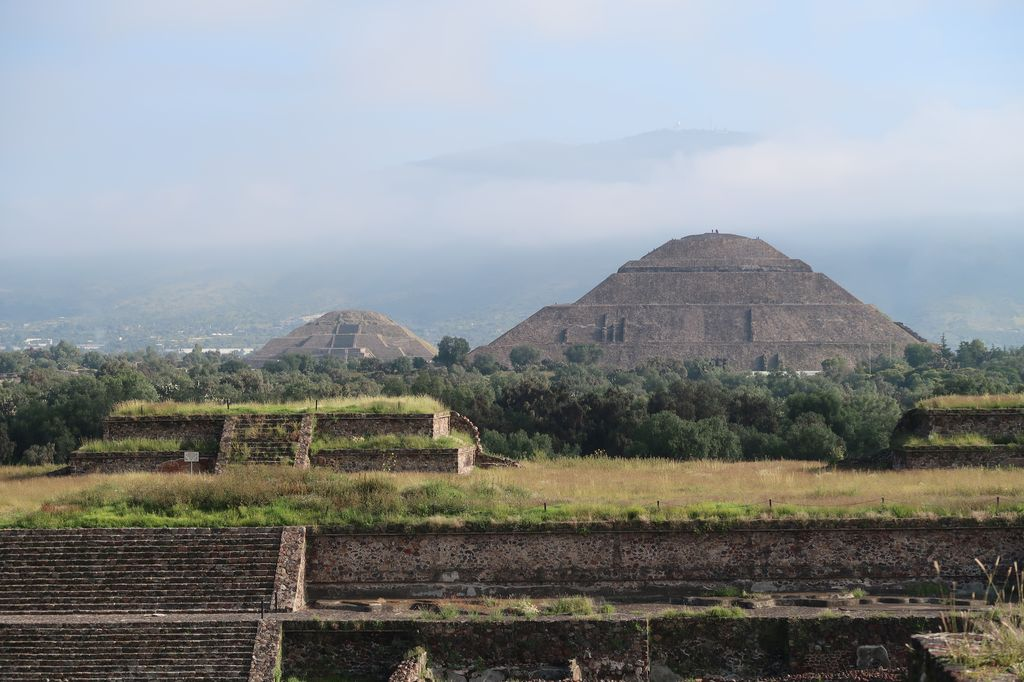
\includegraphics{images/20180930_teotihuacan.JPG}
\caption{Vue sur les deux pyramides de Teotihuacán, impressionnantes.}
\end{figure}

Sur le site partiellement restauré se dressent deux énormes pyramides et
de très nombreuses autres pyramides plus petites. On y retrouve le motif
des serpents à plumes des aztèques, ce qui fait dire à notre guide que
certains éléments religieux aztèques ont été hérités des Teotihuacán,
1000 ans plus tard. Les fouilles archéologiques y sont en standby faute
de moyens, mais on a pu accéder avec Jane à des zones non ouvertes au
public, où se trouvent des symboles pas tout à fait déchiffrés encore,
ou encore une douche antique taillée dans la pierre. La journée passée à
grimper les pyramides (260 marches jusqu'au sommet), se poser des
questions sur la finalité de ce site démesuré, prendre peur quand les
vendeurs ambulants font des cris de jaguars en colère, rechercher des
morceaux de mica par terre (il y en a partout), fouiller la caverne un
peu en dehors du site pour trouver des rasoirs en obsidienne et des
fragments de poterie, était des plus intenses et agréables. Et la
dégustation à la coopérative de tequila, mezcal et autres liqueurs de
cactus a fini de nous achever (et nous faire acheter des souvenirs...) !

Sur les conseils avisés de deux amies de lycée expatriées au Mexique, on
a décidé de passer une nuit à Puebla, à une centaine de kilomètres au
sud-est de Mexico. On a beaucoup aimé se balader dans les rues animées
de la ville, à taille beaucoup plus humaine que la capitale. Le Zocalo
était plein de charme, avec une jolie cathédrale, et à côté la plus
vieille bibliothèque d'Amérique, datant de 1646. On y a aussi visité la
\emph{bling-bling} chapelle du rosaire, complètement recouverte d'or, la
rue des sucreries, et dans un autre registre les tunnels récemment
découverts dans le nord de la ville (dont on a pas vraiment compris
l'utilisation, ni l'âge, ni par qui, ni comment, mais certains disent
qu'ils auraient été utiles aux mexicains lors de la célèbre bataille du
Cinco de Mayo - grande défaite de l'armée française commémorée chaque
année...).

\begin{figure}
\centering
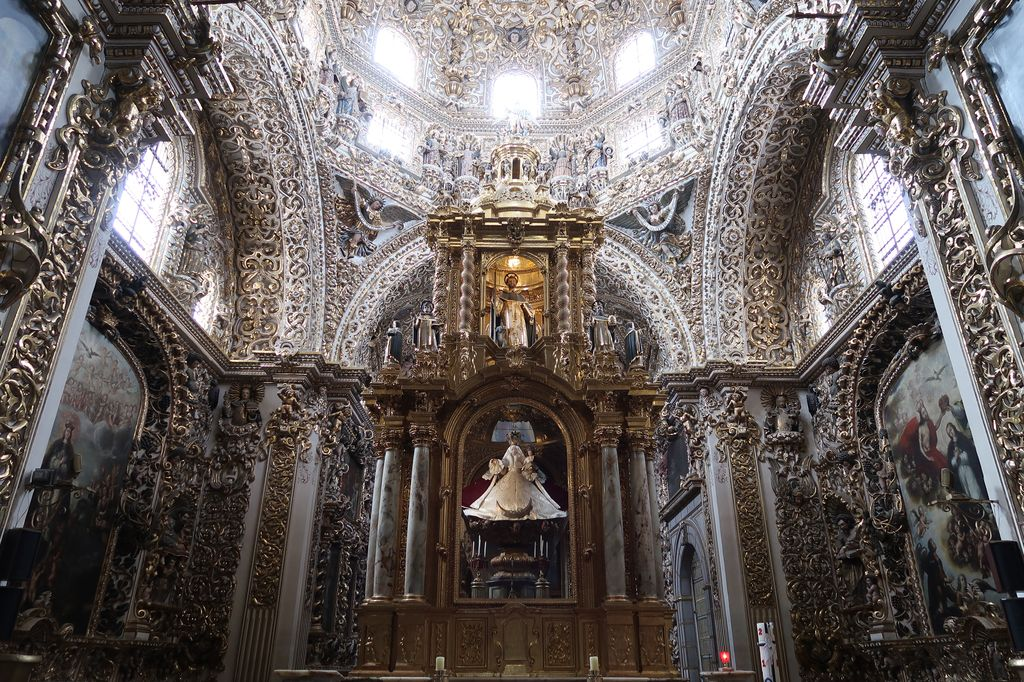
\includegraphics{images/20180930_rosario.JPG}
\caption{Quand on vous dit que la décoration est portée sur le brillant
!}
\end{figure}

A quelques kilomètres de Puebla se trouve la charmante petite ville de
Cholula, encore plus authentique. La principale curiosité locale est
l'église Santa-Maria-de-los-Remedios (très, très fleurie), construite en
haut d'une étrange colline. En effet, ce promontoire n'est rien d'autre
qu'une immense pyramide aztèque (ayant une base plus grande que celle de
Khéops !), elle-même constituée de 7 pyramides en poupées russes !

\begin{figure}
\centering
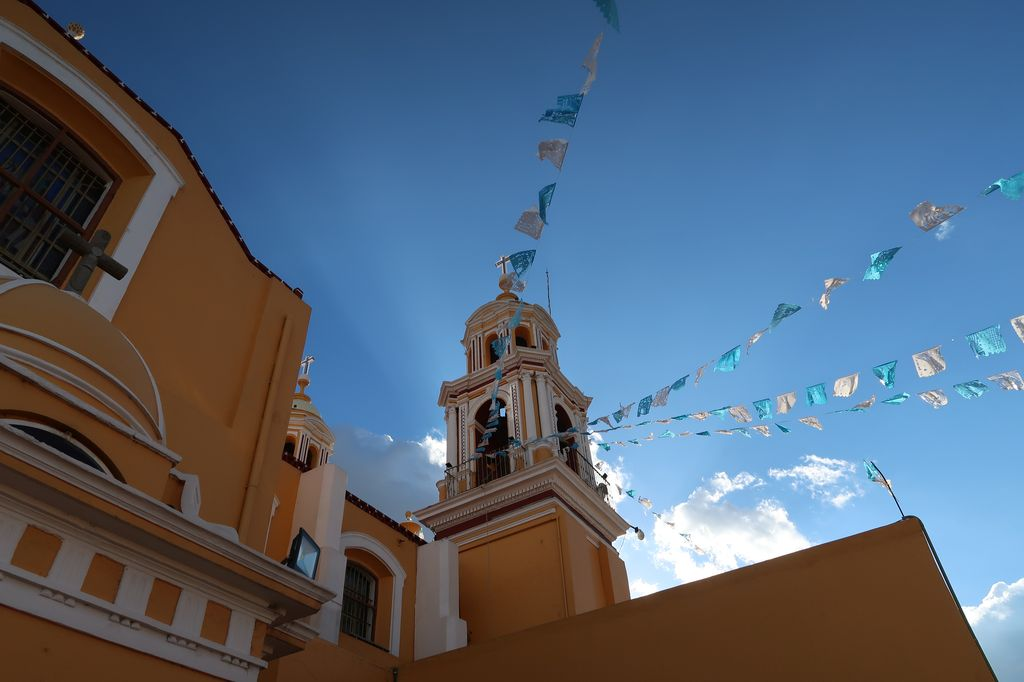
\includegraphics{images/20180930_cholula.JPG}
\caption{}
\end{figure}

Deux semaines à Mexico : on peut dire qu'on en a pris plein les yeux. La
culture aztèque nous a fascinés, et la culture mexicaine est tout aussi
riche ! On vous a pas trop parlé de gastronomie mais on s'est régalés au
fil des stands de rue : tacos en tous genres, gorditas, enchiladas, maïs
grillé au citron et sel ou bouilli à la mayonnaise et parmesan,
sucreries à la confiture de lait, \emph{pulque} à la mangue ou à la
menthe poivrée... j'en ai l'eau à la bouche rien que d'y repenser ! Il y
a tellement de spécialités culinaires au Mexique que c'est le seul pays
de notre voyage que l'on quitte en ayant l'impression de ne pas avoir
goûté à tout ce qui existe !

Mille mercis à Mylène, Cindy et Roman pour vos conseils avisés avant et
pendant le voyage. Vous avez la chance de vivre/d'avoir vécu dans un
pays magnifique, qu'on a hâte d'explorer plus !

On change complètement de registre, de culture, de langue et de météo
pour la prochaine étape : rendez-vous à Vancouver :)

\emph{Elida et Florian}
